\section{Experimental setup and procedure}
\subsection{Method}
To measure the absorption spectra of stainless steel and natural iron, we irradiate the samples with the $14.4keV$ $\gamma$-radiation emitted by a radioactive source. To vary the frequency a motor is used to move the absorber relative to the source (Doppler shift see  \ref{eq:diffdopplershift}). By repeating this measurement for different absorber velocities a spectrum is recorded.\\
\subsection{Setup}
\begin{figure}[hbt]
\centering
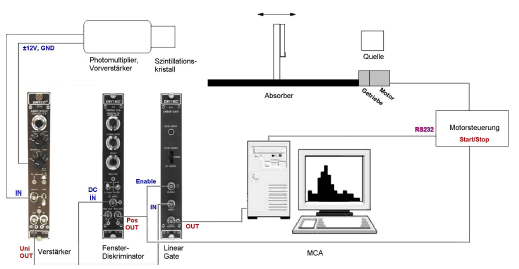
\includegraphics[width=1.0\linewidth]{graphics/Aufbau}
\caption[Setup overview ]{Overview of the experimental setup}
\label{fig:Aufbau}
\end{figure}

The setup consists of the $\gamma$ source, the absorber on a track, the motor used to move the absorber at constant speeds relative to the source and as the photon detector a scintillator is used. The light signal of the scintillator turned into an electric signal by a photomultiplier. This signal is amplified and shaped in the amplifier. The amplifier has two exits, one of which is connected to a single channel analyzer (SCA). If the signal pulse is within an adjustable window the SCA sends a standardized signal and enables the linear gate, which is also connected to the amplifier via a delay to ensure simultaneity of the signals. If the linear gate is enabled when it receives a signal from the amplifier it transmits the amplifier signal to the multichannel analyzer (MCA), which is read out with a Computer. The second output of the SCA is connected to a counter, which also can be read out with the Computer.

\subsection{The source Co-57}
\isotope[57]{Co} decays via electron capture with a branching ratio of $99.8 \%$ and a half life of 270d into an iron in an excited state $\isotope[57]{Fe^*}$. This state decays with a half life of 9ns an branching ratio of $88\%$ into the $14.4$keV excited state which finally decays to the ground state (Branching ratio for $\gamma-decay$ is $10\%$) \ref{fig:principles:Zerfallsschema2}.
\begin{figure}[hbt]
	\centering
	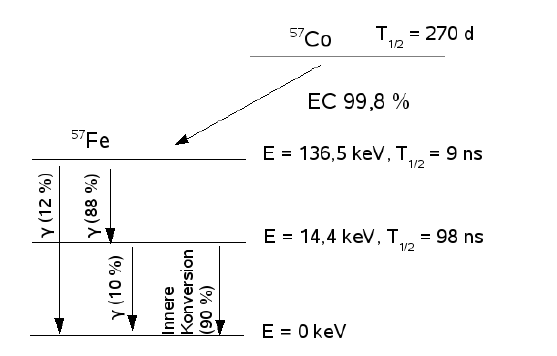
\includegraphics[width=0.5\linewidth]{graphics/Zerfallsschema2}
	\caption[Co-57 decay]{Decay series of Cobalt-57}
	\label{fig:principles:Zerfallsschema2}
\end{figure}
\subsection{Americium sample}
To calibrate the MCA multiple reference samples are used. For this purpose americium is used as a primary source. The americium is shielded in an stainless steel case with a aperture. Attached in front of this aperture a disc with multiple targets(Cu, Rb, Mo, Ag, Ba, and Tb) by rotating the disc one can choose a target (see fig \ref{fig:Americium} ). The radiation of the Americium source excites the target material which in turn starts emitting characteristic x-rays (x-ray fluorescence)\cite{landgraf}. The characteristic lines of the targt samples can be found in fig \ref{fig:Americium_table} and for the americium source in fig
\begin{figure}[H]
\centering
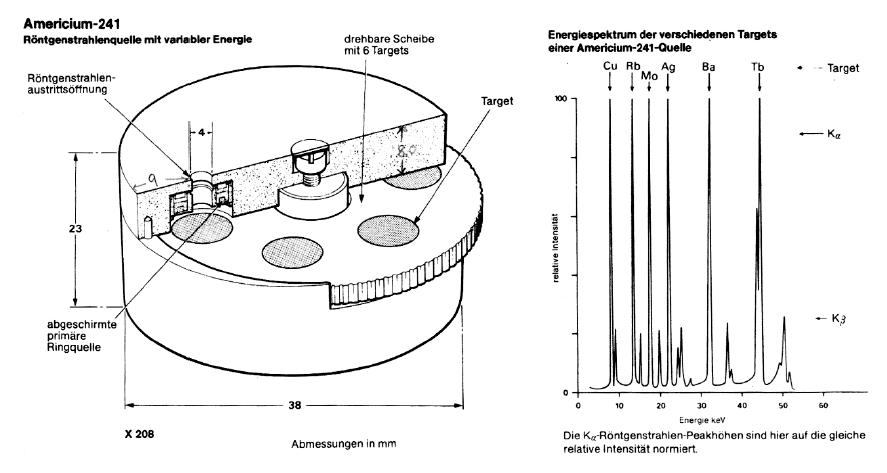
\includegraphics[width=0.7\linewidth]{graphics/Americium}
\caption[Americium sample]{Americium sample with target revolver used as  reference for the MCA calibration\cite{anleitung}}
\label{fig:Americium}
\end{figure}
\begin{figure}[H]
\centering
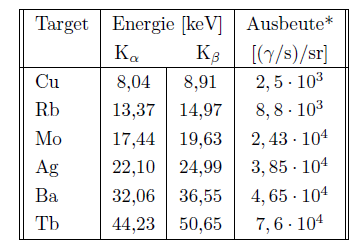
\includegraphics[height=0.2\textheight]{graphics/Americium_table}
\caption{$K_\alpha$ and $K_\beta$ lines of Cu, Rb, Mo, Ag, Ba, and Tb\cite{anleitung}}
\label{fig:Americium_table}
\end{figure}
\begin{figure}[H]
\centering
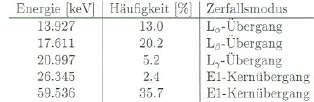
\includegraphics[height=0.2\textheight]{graphics/Amercium_lines}
\caption{The 5 visible lines of the americium source\cite{landgraf}}
\label{fig:Amercium_lines}
\end{figure}

\subsection{Procedure}
\subsubsection{MCA calibration}
First the window size was set to maximum and the spectrum of the cobalt source was recorded.
To identify the $14.4$keV peak of the source, the (known) spectra of Cu, Rb, Mo, Ag, Ba, and Tb are measured for 300s each. The results are used to identify the $14.4$keV peak in the source spectrum. The Window of the SCA was adjusted accordingly, by recording the source spectrum while adjusting the window and repeatedly resetting the recording on the computer. The Window was then adjusted until only the channels of the $14.4keV$ peak get a signal. We chose the settings:
\begin{itemize}
	\item upper level: 1.10
	\item lower level: 0.69
\end{itemize}

\subsubsection{background measurement}
The main source of background are photons of the transition between the $136.5$keV state and the $14.4$kev state (see fig \ref{fig:principles:Zerfallsschema2}) being scatter via Compton scattering in the scintillator and falling in the adjusted SCA window. To measure this background, aluminum plates of different thicknesses (measured with) are used to shield the scintillator. For each plate the event counts were measured over 600s. The plate thicknesses were measured with a caliber. 

\subsubsection{Absorption spectra of stainless steel}
First a rough measurement is made: the absorption was measured for velocities of 0.1 mm/s to 1.1 mm/s (both directions) in steps of 0.1mm/s for 180s. For the finer measurements a measuring time of 300s was chosen.
\subsubsection{Absorption spectra of natural iron}
For natural iron the absorption was measured for absorber speeds between 0.1mm/s and 8mm/s in steps of 0.1mm/s. In a second measurement the range 0.05mm/s to 6.05mm/s was taken, also in steps of 0.1mm/s. The measuring for each velocity was 300s.
\subsubsection{Attenuation through acrylic glass}
The absorber is removed from the setup at the counting rate measured for 900s, once with acrylic glass and once without.
